\documentclass[a4paper,14pt,russian]{extreport}
\usepackage[russian]{babel}

\usepackage{../common/dsturep_ru} % оформление по ДСТУ 3008-95
\usepackage{import}
\usepackage{standalone}
\usepackage{comment}
\usepackage{bbm}

\usepackage{tikz}
\usepackage{tikz-3dplot}
\usetikzlibrary{calc}
\usetikzlibrary{plotmarks}
\usepackage{pgfplots}

%\usepackage{scrextend}
\usepackage{changepage}
\usepackage{caption}
\usepackage{listings}
%\usepackage[title,titletoc]{appendix}
%\usepackage{appendix}
\usepackage{longtable}
%\usepackage{slashbox}
\usepackage{diagbox}
\usepackage{lscape}
\usepackage{algorithmic}
\usepackage{algorithm}

\def\male{male}
\def\female{female}

\bibliographystyle{../common/utf8gost780u}

\usepackage[square,numbers,sort&compress]{natbib}
\renewcommand{\bibnumfmt}[1]{#1.\hfill} % нумерация источников в самом списке — через точку

\def\passYear{2017}
\def\faculty{физико-технический институт}
\def\department{Кафедра информационной безопасности}
\def\departmentHead{Н. В. Грайворонский}
\def\kind{Дипломна робота}
\def\level{магістр}
\def\specialityCode{8.04030101}
\def\specialityTitle{Прикладная математика}
\def\theme{Решение нелинейных уравнений}
\def\gender{female}
\def\mentorGender{male}
\def\course{3}
\def\group{ФИ-41}
\def\name{Лавягина Ольга Алексеевна}
\def\mentorRank{}
\def\mentorName{Стёпочкина Ирина Валерьевна}
\def\reviewerRank{Rank}
\def\reviewerName{Name}
\def\subject{Методы вычислений}



\begin{document}

\import{1_title/}{title.tex}

\clearpage

\pagenumbering{gobble}
%\import{3_abstract/}{main.tex}

%\pagestyle{empty}
%\thispagestyle{empty}
%\tableofcontents

\clearpage
\pagenumbering{arabic}
\pagestyle{fancy}
\setcounter{page}{2}

\clearpage

\chapter{Исходные данные}

В компьютерном практикуме (вариант 8) ищутся корни уравнения
\begin{equation} \label{eq:1}
2x^5 + 3x^2 - 2x - 6 = 0.
\end{equation}

\chapter{Допрограммный этап}

Выпишем все коэффициенты при степенях переменной
$$a_0 = - 6, \, a_1 = - 2, \, a_2 = 3, \, a_3 = 0, \, a_4 = 0, \, a_5 = 2.$$
Проверим условие теоремы Гюа.
Нужно проверить, существует ли $k$ такое, что $0 < k < n$ и $a_k^2 \leq a_{k+1} \cdot a_{k-1}$, то существует хотя бы одна пара комплексно сопряжённых корней.
Проверим это неравенство $a_1^2 = \left( - 2 \right)^2 = 4 > - 6 \cdot 3 =  - 18$ --- не подходит, $a_2^2 = 3^2 = 9 > - 2 \cdot 0 = 0$ --- не подходит, 
$a_3^2 = 0 = 3 \cdot 0 = 0$.
Нашли, что для данного уравнения $k = 3$, то есть существует хотя бы одна пара комплексно сопряжённых корней.

Применим теорему про кольцо.
Введём значения
$$A =
\max \left\{ \left| a_{n - 1} \right|, \, \left| a_{n - 2} \right|, \dotsc, \left| a_0 \right| \right\} =
\max \left\{ 0, 0, 3, 2, 6 \right\} =
6$$
и $B = \max \left\{ \left| a_n \right|, \dotsc, \left| a_1 \right| \right\} = \max \left\{ 2, 0, 0, 3, 2 \right\} = 3$.

Тогда
$$ \left| x \right| <
\frac{ \left| a_n \right| + A}{ \left| a_n \right| } =
\frac{2 + 6}{2} =
\frac{4}{2} =
2 =
R$$
--- больший радиус кольца.

С другой стороны
$$ \left| x \right| >
\frac{ \left| a_0 \right| }{ \left| a_0 \right| + B} =
\frac{6}{6 + 3} =
\frac{6}{9} =
\frac{2}{3} =
r$$
--- меньший радиус кольца.

Получили, что
$$r =
\frac{2}{3} <
\left| x \right| <
2 =
R.$$

Применим теорему про верхнюю границу.
Введём величину
$$B = \max \left| a_i \right| = 6, \,
m = \max i = 0, \,
a_i < 0.$$
Тогда положительные корни ограничены сверху величиной
$$x^{+} <
1 + \sqrt[n - m]{ \frac{B}{a_n}} =
1 + \sqrt[5 - 0]{ \frac{6}{2}} =
1 + \sqrt[5]{3} \approx
1 + 1.25 =
2.25.$$

Теорема про кольцо дала лучший результат на верхнюю границу положительных корней уравнения.

По теореме про верхнюю границу получили значение $R = 2.25$.
Рассмотрим уравнение
$$P \left( \frac{1}{y} \right) =
2 \left( \frac{1}{y} \right)^5 + 3 \left( \frac{1}{y} \right)^2 - 2 \cdot \frac{1}{y} - 6 =
0.$$
Домножим это уравнение на $y^5$.
Получаем
$$y^n P \left( \frac{1}{y} \right) =
2 + 3y^3 - 2y^4 - 6y^5 = 0.$$
Умножим полученное уравнение на $ \left( - 1 \right) $.
Получим $6y^5 + 2y^4 - 3y^3 - 2 = 0$.
Применим теорему про верхнюю границу.
Введём величину
$$B = \max \left| a_i \right| = 3, \,
m = \max i = 3, \,
a_i < 0.$$
Тогда положительные корни ограничены сверху величиной
$$y^{+} <
1 + \sqrt[n - m]{ \frac{B}{a_n}} =
1 + \sqrt[5 - 3]{ \frac{3}{6}} =
1 + \sqrt{ \frac{1}{2}} \approx
1 + 0.71 =
2.71 =
R_1.$$
Тогда
$$ \frac{1}{R_1} =
\frac{1}{2.71} \approx
0.74 <
x^{+} <
2.25 =
R.$$

Теорема про верхнюю границу дала лучшее ограничение снизу для положительных корней.

Применим другую замену:
$$P \left( - y \right) =
2 \left( - y \right)^5 + 3\left( - y \right)^2 - 2 \left( - y \right) - 6 =
- 2y^5 + 3y^2 + 2y - 6 =
0.$$
Умножаем это уравнение на $ \left( - 1 \right) $.
Получаем $2y^5 - 3y^2 - 2y + 6 = 0$.
Вводим величину $B = \max \left| a_i \right| = 3, \, m = \max i = 2, \, a_i < 0$.
Тогда положительные корни уравнения $P \left( - y \right) = 0$ ограничены сверху величиной
$$y^{+} <
1 + \sqrt[n - m]{ \frac{B}{a_n}} =
1 + \sqrt[5 - 2]{ \frac{3}{2}} =
1 + \sqrt[3]{1.5} \approx
1 + 1.14 =
2.14 =
R_2.$$

Сделаем последнюю замену
$$P \left( - \frac{1}{y} \right) =
2 \left( \frac{1}{y} \right)^5 - 3 \left( \frac{1}{y} \right)^2 - 2 \cdot \frac{1}{y} + 6 =
0.$$
Умножим полученное уравнение на $y^5$.
Получим $2 - 3y^3 -2y^4 + 6y^5 = 0$.
Применим для него теорему про верхнюю границу.
Введём величину
$$B = \max \left| a_i \right| = 3, \,
m = \max i = 3, \,
a_i < 0.$$
Тогда положительные корни ограничены сверху величиной
$$y^{+} <
1 + \sqrt[n - m]{ \frac{B}{a_n}} =
1 + \sqrt[5 - 3]{ \frac{3}{6}} =
1 + \sqrt{0.5} \approx
1 + 0.71 =
1.71 =
R_3.$$

Для исходного уравнения отрицательные корни будут ограничены значениями
$$- R_2 =
- 2.14 <
x^{-} <
- \frac{1}{R_3} 
- \frac{1}{1.71} =
- 0.58.$$

Теорема про кольцо дала лучшее ограничение снизу отрицательных корней, но худшее ограничение сверху для них.
Если объединить 2 результата, получим $- 2 < x^{-} < - 0.58$.

Применим теорему Лагранжа.
Выписываем полином
$$P \left( x \right) = 2x^5 + 3x^2 - 2x - 6.$$
Раскладываем полином на две части $P \left( x \right) = F \left( x \right) + \Phi \left( x \right) $,
где $F \left( x \right) = 2x^5 + 3x^2 - 2x - 6$ содержит все подряд старшие компоненты с положительными коэффициентами и все отрицательные,
$ \Phi \left( x \right) = 0$ содержит все остальные.

Если существует $ \alpha $ такое, что $F \left( \alpha \right) \geq 0$, то $x^{+} < \alpha $.
Подходит значение $ \alpha = 1.2$.
Проверяем
$F \left( \alpha \right) =
F \left( 1.2 \right) =
2 \cdot \left( 1.2 \right)^5 + 3 \left( 1.2 \right)^2 - 2 \cdot 1.2 - 6 \approx 0.9 > 0$.

Получили $ \frac{2}{3} < x^{+} < 1.2$.

Корни уравнения были найдены с помощью \href{http://www.wolframalpha.com}{WolframAlpha}, построен график (рис. \ref{fig:plot}).

\begin{figure}[h!]
  \centering
  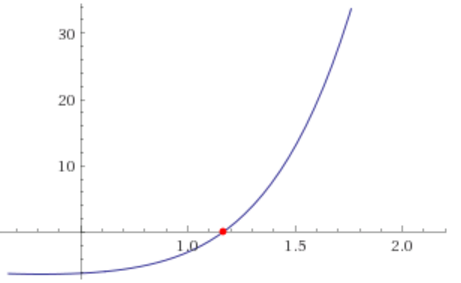
\includegraphics[width=.3\textwidth]{plot.png}
  \caption{График полинома $f \left( x \right) = 2x^5 + 3x^2 - 2x - 6$}
\label{fig:plot}
\end{figure}

Красной точкой на графике отмечен корень уравнения \ref{eq:1}.
По теоремам нашли, что он лежит на промежутке
$$ \left[ a, b \right] = \left[ \frac{2}{3}, 1.2 \right].$$

\chapter{Листинг программы}

Листинг файла utils.py
\lstset{inputencoding=utf8, extendedchars=\true}
\lstinputlisting[language=python,
                 basicstyle=\ttfamily\scriptsize]{../code/utils.py}

Листинг программы уточнения корней по методу бисекции
\lstset{inputencoding=utf8, extendedchars=\true}
\lstinputlisting[language=python,
                 basicstyle=\ttfamily\scriptsize]{../code/bisection.py}

Листинг программы уточнения корней по методу хорд
\lstset{inputencoding=utf8, extendedchars=\true}
\lstinputlisting[language=python,
                 basicstyle=\ttfamily\scriptsize]{../code/horde.py}

Листинг программы уточнения корней по методу Ньютона (касательных)
\lstset{inputencoding=utf8, extendedchars=\true}
\lstinputlisting[language=python,
                 basicstyle=\ttfamily\scriptsize]{../code/newton.py}

\chapter{Результаты работы программы}

Результаты метода бисекции
\lstset{inputencoding=utf8, extendedchars=\true}
\lstinputlisting[language=bash,
                 basicstyle=\ttfamily\scriptsize]{../code/bisection_result.txt}

Результаты метода хорд с критерием завершения процесса $ \left| f \left( c \right) \right| < \varepsilon $
\lstset{inputencoding=utf8, extendedchars=\true}
\lstinputlisting[language=bash,
                 basicstyle=\ttfamily\scriptsize]{../code/horde_result.txt}

Результаты метода хорд с критерием завершения процесса
$$\left| c - c_{previous} \right| < \varepsilon $$
\lstset{inputencoding=utf8, extendedchars=\true}
\lstinputlisting[language=bash,
                 basicstyle=\ttfamily\scriptsize]{../code/horde_result_difference.txt}

Результаты метода Ньютона (касательных) с критерием завершения процесса $ \left| f \left( x_0 \right) \right| < \varepsilon $
\lstset{inputencoding=utf8, extendedchars=\true}
\lstinputlisting[language=bash,
                 basicstyle=\ttfamily\scriptsize]{../code/newton_result.txt}

Результаты метода Ньютона (касательных) с критерием завершения процесса $ \left| x_{0_{previous}} - x_0 \right| < \varepsilon $
\lstset{inputencoding=utf8, extendedchars=\true}
\lstinputlisting[language=bash,
                 basicstyle=\ttfamily\scriptsize]{../code/newton_result_difference.txt}

\chapter*{Выводы}
\addcontentsline{toc}{chapter}{Выводы}

С помощью метода бисекции корень заданного уравнения был получен на 16-й итерации,
с помощью метода хорд --- на 13-й,
а с помощью метода Ньютона (касательных) ---на четвёртой.

Для метода бисекции было обнаружено, что при увеличении длины отрезка количество итераций возрастает, но при уменьшении длины отрезка практически не меняется.
Так, для отрезка $ \left[ 1.1, 1.2 \right] $ результат был получен на 14-й итерации.

Метод хорд даёт результат гораздо быстрее.
Для отрезка $ \left[ 1.1, 1.2 \right] $ результат был получен за на четвёртой итерации.

Преимуществом метода Ньютона (касательных) является его быстрая сходимость.
Для данного метода необходимо знать начальное приближение, а не границы интервала, в котором находится корень.
Недостатком является то, что метод может зацикливаться (в данном случае, например, при $x_0 = 1$).

\end{document}
